\documentclass[a4paper, 12pt]{article}

\usepackage[utf8]{inputenc}
\usepackage{amsmath}
\usepackage[]{amsfonts}
\usepackage[]{graphicx}

\title{CS231A Lecture Notes 1: Camera Models}
\author{Silvio Savarese and Kenji Hata}
\date{}

\renewcommand\emph{\textbf}

\begin{document}

\maketitle

\section{Introduction}
The camera is one of the most essential tools in computer vision. It is the mechanism by which we can record the world around us and use its output - photographs - for various applications. Therefore, one question we must ask in introductory computer vision is: how do we model a camera?

\section{Pinhole cameras}
\begin{figure}[h!]
\centering
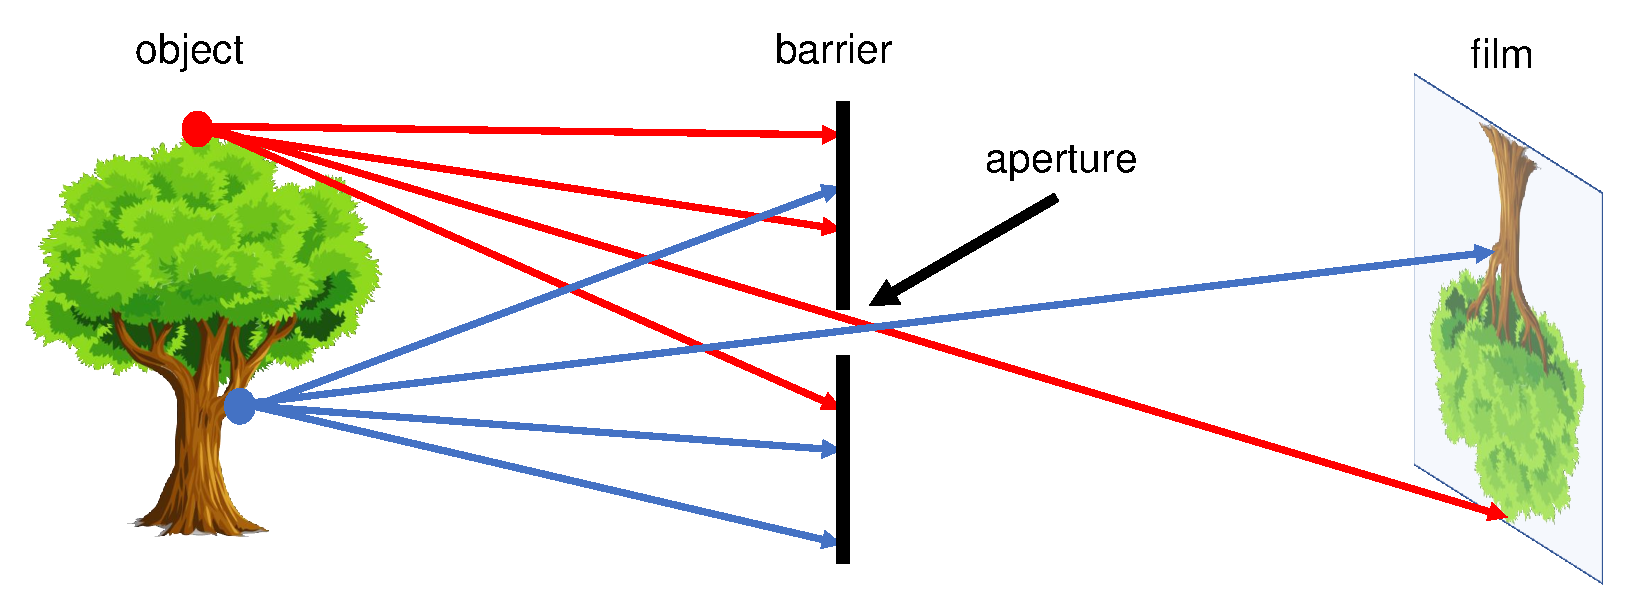
\includegraphics[width=0.8\textwidth]{figures/1-1.pdf}
\caption{A simple working camera model: the pinhole camera model.}
\label{fig:simpleCamera}
\end{figure}
Let's design a simple camera system -- a system that can record an image of an object or scene in the 3D world. This camera system can be designed by placing a barrier with a small aperture between the 3D object and a photographic film or sensor. As Figure~\ref{fig:simpleCamera} shows, each point on the 3D object emits multiple rays of light outwards. Without a barrier in place, every point on the film will be influenced by light rays emitted from every point on the 3D object. Due to the barrier, only one (or a few) of these rays of light passes through the aperture and hits the film. Therefore, we can establish a one-to-one mapping between points on the 3D object and the film. The result is that the film gets exposed by an ``image" of the 3D object by means of this mapping. This simple model is known as the \emph{pinhole camera model}.

\begin{figure}[h!]
\centering
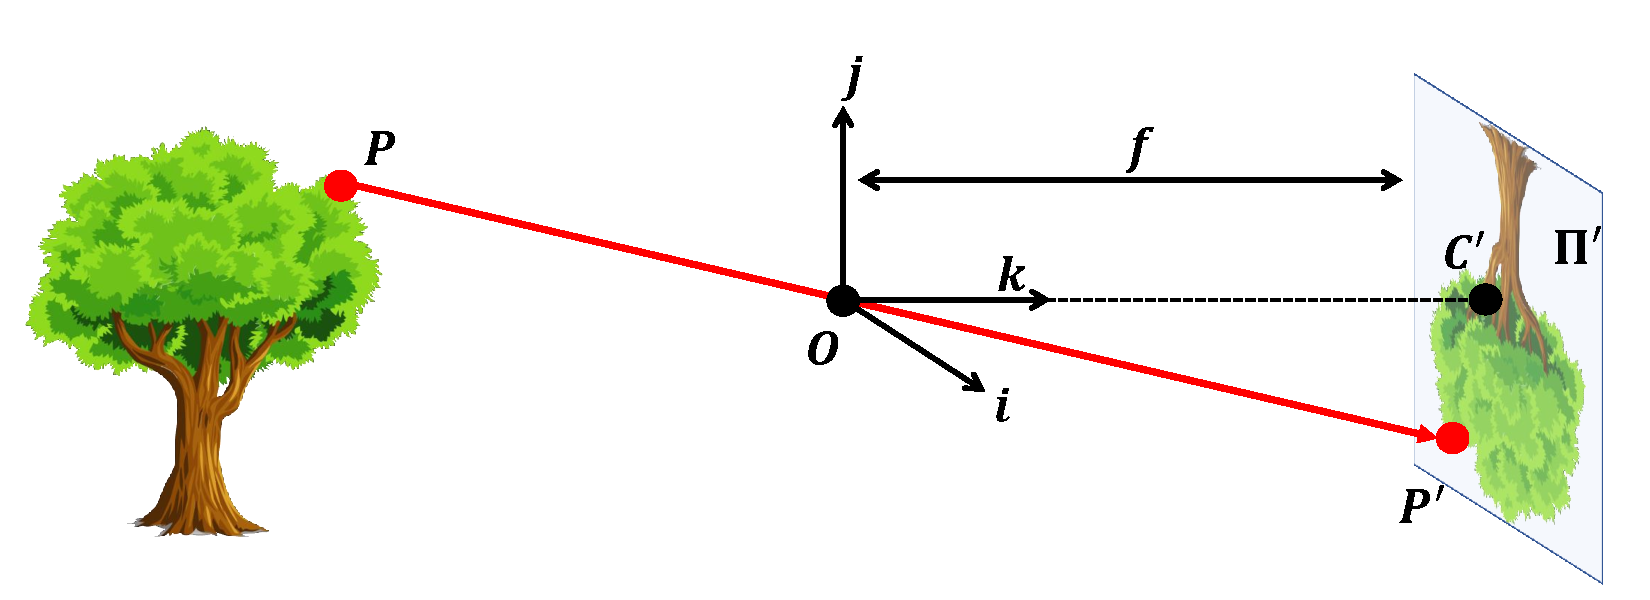
\includegraphics[width=0.8\textwidth]{figures/1-2.pdf}
\caption{A formal construction of the pinhole camera model.}
\label{fig:pinholeCamera}
\end{figure}
A more formal construction of the pinhole camera is show in Figure~\ref{fig:pinholeCamera}. In this construction, the film is commonly called the \emph{image or retinal plane}. The aperture is referred to as the \emph{pinhole} $O$ or \emph{center of the camera}. The distance between the image plane and the pinhole $O$ is the \emph{focal length} $f$. Sometimes, the retinal plane is placed between $O$ and the 3D object at a distance $f$ from $O$. In this case, it is called the \emph{virtual image} or \emph{virtual retinal plane}. Note that the projection of the object in the image plane and the image of the object in the virtual image plane are identical up to a scale (similarity) transformation.

Now, how do we use pinhole cameras? Let $P = \begin{bmatrix}x & y & z\end{bmatrix}^T$ be a point on some 3D object visible to the pinhole camera. $P$ will be mapped or \textbf{projected} onto the image plane $\Pi'$, resulting in point\footnote{Throughout the course notes, let the prime superscript (e.g. $P'$) indicate that this point is a projected or complementary point to the non-superscript version. For example, $P'$ is the projected version of $P$.} $P' = \begin{bmatrix}x' & y'\end{bmatrix}^T$. Similarly, the pinhole itself can be projected onto the image plane, giving a new point $C'$. 

Here, we can define a coordinate system $\begin{bmatrix}i & j & k\end{bmatrix}$ centered at the pinhole $O$ such that the axis $k$ is perpendicular to the image plane and points toward it. This coordinate system is often known as the \emph{camera reference system} or \emph{camera coordinate system}. The line defined by $C'$ and $O$ is called the \emph{optical axis} of the camera system.

Recall that point $P'$ is derived from the projection of 3D point $P$ on the image plane $\Pi'$. Therefore, if we derive the relationship between 3D point $P$ and image plane point $P'$, we can understand how the 3D world imprints itself upon the image taken by a pinhole camera. Notice that triangle $P'C'O$ is similar to the triangle formed by $P$, $O$ and $(0,0,z)$. Therefore, using the law of similar triangles we find that 

\begin{equation}
    P' = \begin{bmatrix}x'&y'\end{bmatrix}^T = \begin{bmatrix}f\frac{x}{z} & f\frac{y}{z}\end{bmatrix}^T
\end{equation}

Notice that one large assumption we make in this pinhole model is that the aperture is a single point. In most real world scenarios, however, we cannot assume the aperture can be infinitely small. Thus, what is the effect of aperture size? 

\begin{figure}[h!]
\centering
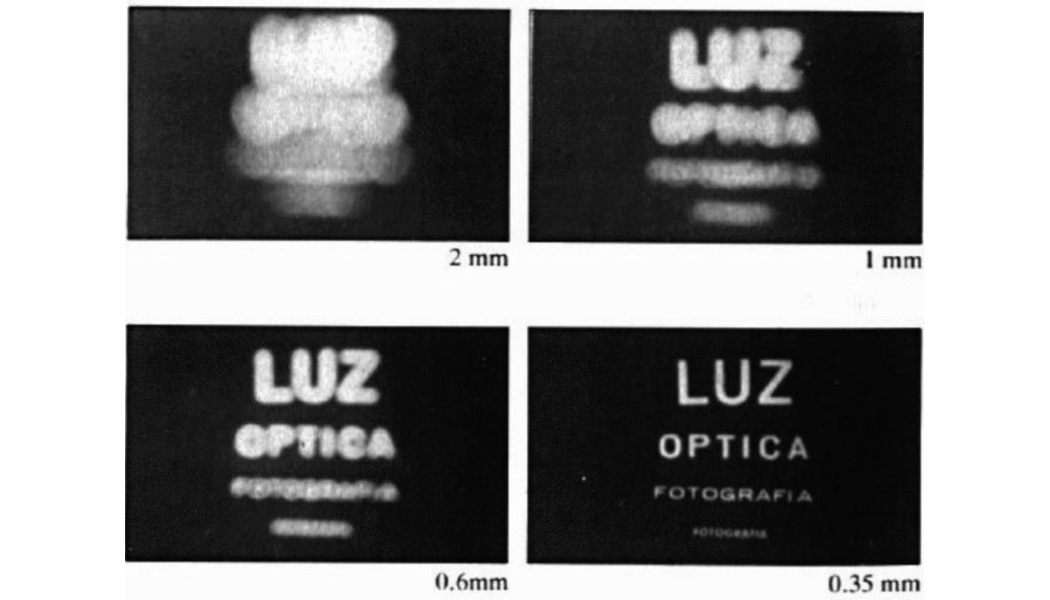
\includegraphics[width=0.8\textwidth]{figures/1-3.pdf}
\caption{The effects of aperture size on the image. As the aperture size decreases, the image gets sharper, but darker.}
\label{fig:apertureSize}
\end{figure}

As the aperture size increases, the number of light rays that passes through the barrier consequently increases. With more light rays passing through, then each point on the film may be affected by light rays from multiple points in 3D space, blurring the image. Although we may be inclined to try to make the aperture as small as possible, recall that a smaller aperture size causes less light rays to pass through, resulting in crisper but darker images. Therefore, we arrive at the fundamental problem presented by the pinhole formulation: can we develop cameras that take crisp and bright images?

\section{Cameras and lenses}
\begin{figure}[h!]
\centering
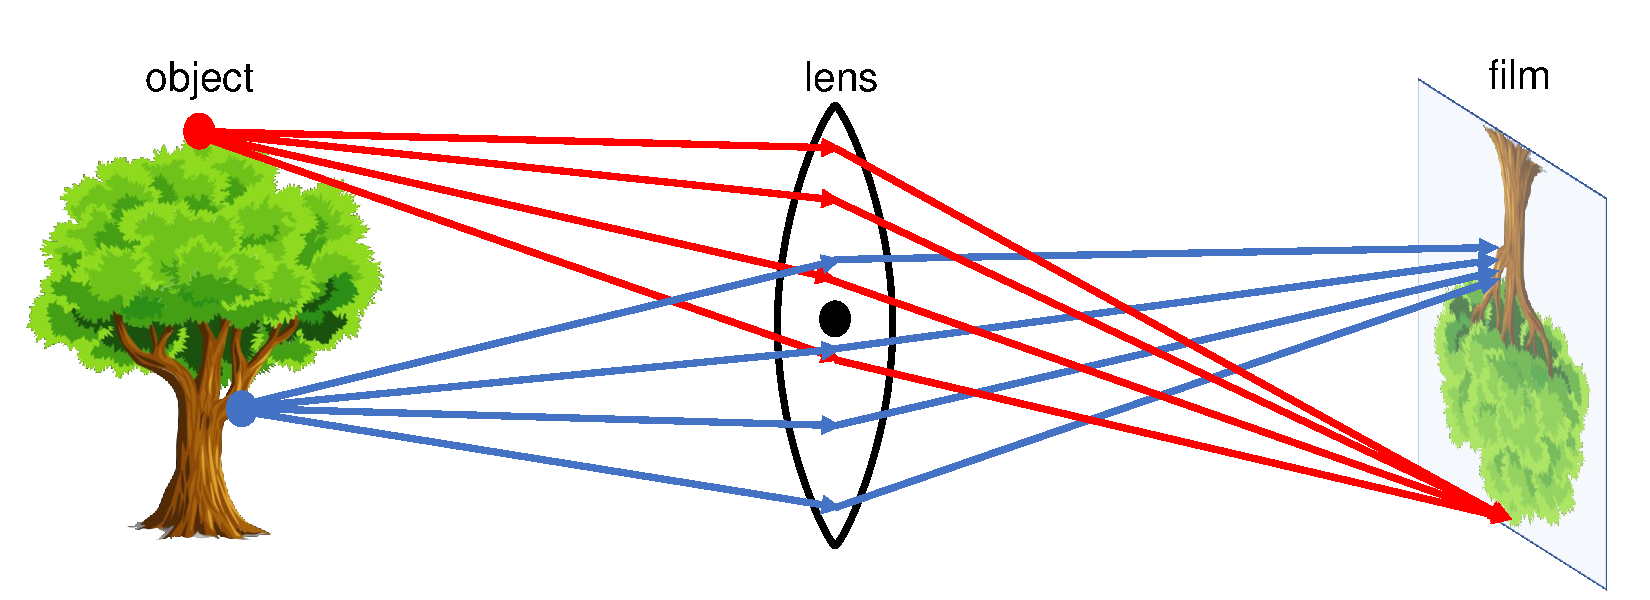
\includegraphics[width=0.8\textwidth]{figures/1-4.pdf}
\caption{A setup of a simple lens model. Notice how the rays of the top point on the tree converge nicely on the film. However, a point at a different distance away from the lens results in rays not converging perfectly on the film.}
\label{fig:lens}
\end{figure}

In modern cameras, the above conflict between crispness and brightness is mitigated by using \emph{lenses}, devices that can focus or disperse light. If we replace the pinhole with a lens that is both properly placed and sized, then it satisfies the following property: all rays of light that are emitted by some point $P$ are refracted by the lens such that they converge to a single point $P'$ in the image plane. Therefore, the problem of the majority of the light rays blocked due to a small aperture is removed (Figure~\ref{fig:lens}). However, please note that this property does not hold for all 3D points, but only for some specific point $P$. Take another point $Q$ which is closer or further from the image plane than $P$. The corresponding projection into the image will be blurred or out of focus. Thus, lenses have a specific distance for which objects are ``in focus". This property is also related to a photography and computer graphics concept known as depth of field, which is the effective range at which cameras can take clear photos.

\begin{figure}[h!]
\centering
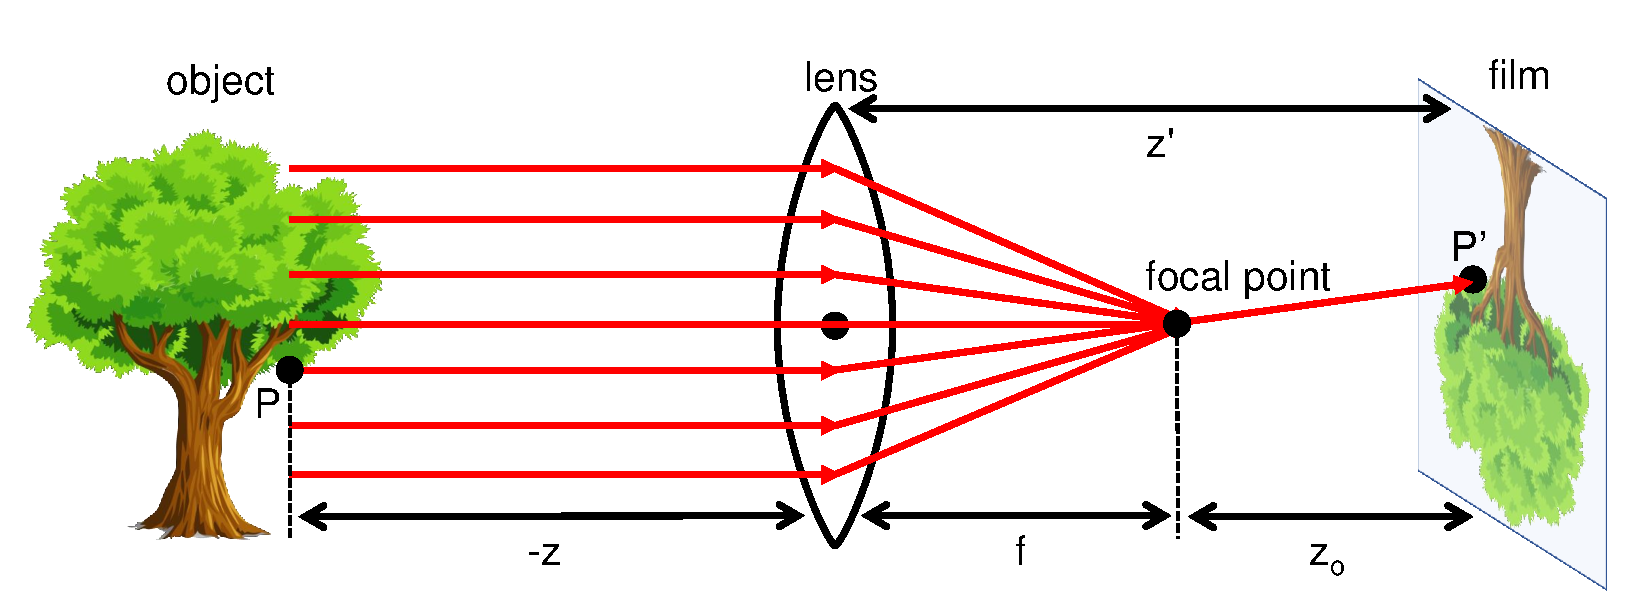
\includegraphics[width=0.8\textwidth]{figures/1-5.pdf}
\caption{Lenses focus light rays parallel to the optical axis into the focal point. Furthermore, this setup illustrates the paraxial refraction model, which helps us find the relationship between points in the image plane and the 3D world in cameras with lenses.}
\label{fig:paraxial}
\end{figure}

Camera lenses have another interesting property: they focus all light rays traveling parallel to the optical axis to one point known as the \emph{focal point} (Figure~\ref{fig:paraxial}). The distance between the focal point and the center of the lens is commonly referred to as the \emph{focal length} $f$. Furthermore, light rays passing through the center of the lens are not deviated. We thus can arrive at a similar construction to the pinhole model that relates a point $P$ in 3D space with its corresponding point $P'$ in the image plane. 

\begin{equation}
    P' = \begin{bmatrix}x'\\ y'\end{bmatrix} = \begin{bmatrix}z'\frac{x}{z} \\ z'\frac{y}{z}\end{bmatrix}
\end{equation}

The derivation for this model is outside the scope of the class. However, please notice that in the pinhole model $z' = f$, while in this lens-based model, $z' = f+z_0$.  Additionally, since this derivation takes advantage of the paraxial or ``thin lens" assumption\footnote{For the angle $\theta$ that incoming light rays make with the optical axis of the lens, the paraxial assumption substitutes $\theta$ for any place $\sin(\theta)$ is used. This approximation of $\theta$ for $\sin\theta$ holds as $\theta$ approaches 0.}, it is called the \textbf{paraxial refraction model}.

\begin{figure}[h!]
\centering
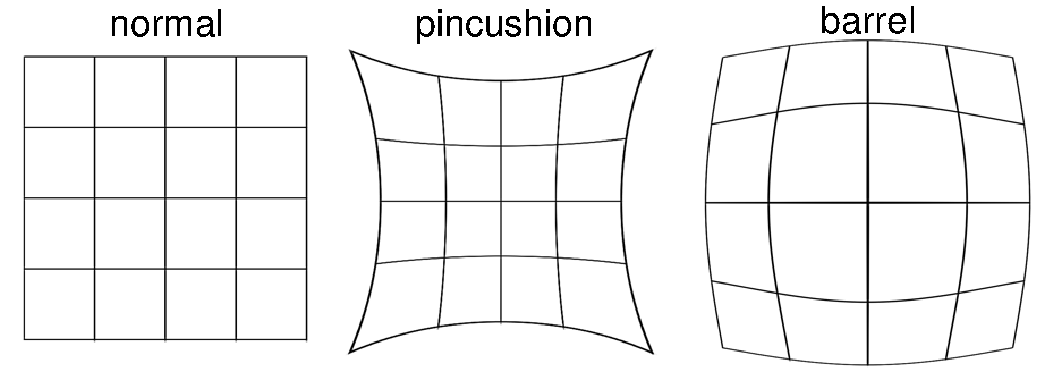
\includegraphics[width=0.8\textwidth]{figures/1-6.pdf}
\caption{Demonstrating how pincushion and barrel distortions affect images.}
\label{fig:distortion}
\end{figure}

Because the paraxial refraction model approximates using the thin lens assumption, a number of aberrations can occur. The most common one is referred to as \emph{radial distortion}, which causes the image magnification to decrease or increase as a function of the distance to the optical axis. We classify the radial distortion as \emph{pincushion distortion} when the magnification increases and \emph{barrel distortion}\footnote{Barrel distortion typically occurs when one uses fish-eye lenses.} when the magnification decreases. Radial distortion is caused by the fact that different portions of the lens have differing focal lengths.

\section{Going to digital image space}
In this section, we will discuss the details of the parameters we must account for when modeling the projection from 3D space to the digital images we know. All the results derived will use the pinhole model, but they also hold for the paraxial refraction model.

As discussed earlier, a point $P$ in 3D space can be mapped (or projected) into a 2D point $P'$ in the image plane $\Pi'$. This $\mathbb{R}^3 \rightarrow \mathbb{R}^2$ mapping is referred to as a \emph{projective transformation}. This projection of 3D points into the image plane does not directly correspond to what we see in actual digital images for several reasons. First, points in the digital images are, in general, in a different reference system than those in the image plane. Second, digital images are divided into discrete pixels, whereas points in the image plane are continuous. Finally, the physical sensors can introduce non-linearity such as distortion to the mapping. To account for these differences, we will introduce a number of additional transformations that allow us to map any point from the 3D world to pixel coordinates.

Image coordinates have their origin $C'$ at the image center where the $k$ axis intersects the image plane. On the other hand, digital images typically have their origin at the lower-left corner of the image. Thus, 2D points in the image plane and 2D points in the image are offset by a translation vector $\begin{bmatrix}c_x, c_y\end{bmatrix}^T$. To accommodate this change of coordinate systems, the mapping now becomes:

\begin{equation}
    P' = \begin{bmatrix}x'\\y'\end{bmatrix} = \begin{bmatrix}f\frac{x}{z}+c_x \\ f\frac{y}{z}+c_y\end{bmatrix}
\end{equation}

The next effect we must account for that the points in digital images are expressed in pixels, while points in image plane are represented in physical measurements (e.g. centimeters). In order to accommodate this change of units, we must introduce two new parameters $k$ and $l$. These parameters, whose units would be something like $\frac{\mathrm{pixels}}{\mathrm{cm}}$, correspond to the change of units in the two axes of the image plane. Note that $k$ and $l$ may be different because the aspect ratio of the unit element is not guaranteed to be one. If $k=l$, we often say that the camera has \emph{square pixels}. We adjust our previous mapping to be

\begin{equation}
    P' = \begin{bmatrix}x'\\y'\end{bmatrix} = \begin{bmatrix}fk\frac{x}{z}+c_x \\ fl\frac{y}{z}+c_y\end{bmatrix} = \begin{bmatrix}\alpha\frac{x}{z}+c_x \\ \beta\frac{y}{z}+c_y\end{bmatrix}
    \label{eq:finalImage}
\end{equation}

Is there a better way to represent this projection from $P\rightarrow P'$? If this projection is a linear transformation, then it can be represented as a product of a matrix and the input vector (in this case, it would be $P$. However, from Equation~\ref{eq:finalImage}, we see that this projection $P\rightarrow P'$ is not linear, as the operation divides one of the input parameters (namely $z$). Still, representing this projection as a matrix-vector product would be useful for future derivations. Therefore, can we represent our transformation as a matrix-vector product despite its nonlinearity?

One way to get around this problem is to change the coordinate systems. For example, we introduce a new coordinate, such that any point $P' =(x',y')$ becomes $(x',y',1)$. Similarly, any point $P =(x,y,z)$ becomes $(x,y,z,1)$. This augmented space is referred to as the \emph{homogenous coordinate system}. As demonstrated previously, to convert some Euclidean vector $(v_1,...,v_n)$ to homogenous coordinates, we simply append a 1 in a new dimension to get $(v_1,...,v_n,1)$. Note that the equality between a vector and its homogenous coordinates only occurs when the final coordinate equals one. Therefore, when converting back from arbitrary homogenous coordinates $(v_1,  ... , v_n , w)$, we get Euclidean coordinates $(\frac{v_1}{w},...,\frac{v_n}{w})$. Using homogenous coordinates, we can formulate
\begin{equation}
    P_h' = \begin{bmatrix}\alpha x + c_xz\\\beta y + c_yz \\ z\end{bmatrix} = 
    \begin{bmatrix}
    \alpha & 0 & c_x & 0\\
    0 & \beta & c_y & 0 \\ 
    0 & 0 & 1 & 0
    \end{bmatrix}
    \begin{bmatrix}x\\y\\z\\1\end{bmatrix} =     \begin{bmatrix}
    \alpha & 0 & c_x & 0\\
    0 & \beta & c_y & 0 \\ 
    0 & 0 & 1 & 0
    \end{bmatrix} P_h
    \label{eq:homogenous}
\end{equation}

From this point on, assume that we will work in homogenous coordinates, unless stated otherwise. We will drop the $h$ index, so any point $P$ or $P'$ can be assumed to be in homogenous coordinates. As seen from Equation~\ref{eq:homogenous}, we can represent the relationship between a point in 3D space and its image coordinates by a matrix vector relationship:
\begin{equation}
    P' = \begin{bmatrix}x'\\y'\\ z\end{bmatrix}=\begin{bmatrix}
    \alpha & 0 & c_x & 0\\
    0 & \beta & c_y & 0 \\ 
    0 & 0 & 1 & 0
    \end{bmatrix}\begin{bmatrix}x\\y\\z\\1\end{bmatrix}=
    \begin{bmatrix}
    \alpha & 0 & c_x & 0\\
    0 & \beta & c_y & 0 \\ 
    0 & 0 & 1 & 0
    \end{bmatrix}P = MP 
    \label{eq:canonical}
    % = K\begin{bmatrix} I&0\end{bmatrix}P
\end{equation}
We can decompose this transformation a bit further into 
\begin{equation}
P' = MP = \begin{bmatrix}
    \alpha & 0 & c_x \\
    0 & \beta & c_y  \\ 
    0 & 0 & 1 
    \end{bmatrix}\begin{bmatrix}I & 0\end{bmatrix}P = K\begin{bmatrix}I & 0\end{bmatrix}P
    \label{eq:decomposedHomogenousTransform}
\end{equation}
The matrix $K$ is often referred to as the \emph{camera matrix}. This matrix contains some of the critical parameters that are useful to characterize a camera model. Two parameters are currently missing from our formulation: \emph{skewness} and \emph{distortion}. We often say that an image is skewed when the camera coordinate system is skewed. In this case, the angle between the two axes are slightly larger or smaller than 90 degrees. Most cameras have zero-skew, but some degree of skewness may occur because of sensor manufacturing errors. Deriving the new camera matrix accounting for skewness is outside the scope of this class and we give it to you below:
\begin{equation}
K = \begin{bmatrix}x'\\y'\\ z\end{bmatrix}=\begin{bmatrix}
    \alpha & -\alpha\cot\theta & c_x \\
    0 & \frac{\beta}{\sin\theta} & c_y  \\ 
    0 & 0 & 1 
    \end{bmatrix}
\end{equation}
Most methods that we introduce in this class ignore distortion effects. Therefore, our final camera matrix has 5 degrees of freedom: 2 for focal length, 2 for offset, and 1 for skewness. 

So far, we have described a mapping between a point $P$ in the 3D camera reference system to a point $P'$ in the 2D image plane. But what if the information about the 3D world is available in a different coordinate system? Then, we need to include an additional transformation that relates points from the world reference system to the camera reference system. This transformation is captured by a rotation matrix $R$ and translation vector $T$. Therefore, given a point in a world reference system $P_w$, we can compute its camera coordinates as follows:
\begin{equation}
P = \begin{bmatrix}R&T\\0&1\end{bmatrix} P_w
\end{equation}
Substituting this in equation (\ref{eq:decomposedHomogenousTransform}) and simplifying gives
\begin{equation}
P' = K\begin{bmatrix}R&T\end{bmatrix}P_w = MP_w
\label{eq:cameramatrix}
\end{equation}

This completes the mapping from a 3D point $P$ in an arbitrary world reference system to the image plane. We see that the projection matrix $M$ consists of two types of parameters: \emph{intrinsic} and \emph{extrinsic} parameters. All parameters contained in the camera matrix $K$ are the intrinsic parameters, which change as the type of camera changes. The extrinsic paramters include the rotation and translation, which do not depend on the camera's build. Overall, we find that the $3\times4$ projection matrix $M$ has 11 degrees of freedom: 5 from the intrinsic camera matrix, 3 from extrinsic rotation, and 3 from extrinsic translation.

\section{Camera Calibration}
To precisely know the transformation from the real, 3D world into digital images requires prior knowledge of many of the camera's intrinsic parameters. If given an arbitrary camera, we may or may not have access to these parameters. We do, however, have access to the images the camera takes. Therefore, can we find a way to deduce them from images? This problem of estimating the extrinsic and intrinsic camera parameters is known as \emph{camera calibration}.

\begin{figure}[h!]
\centering
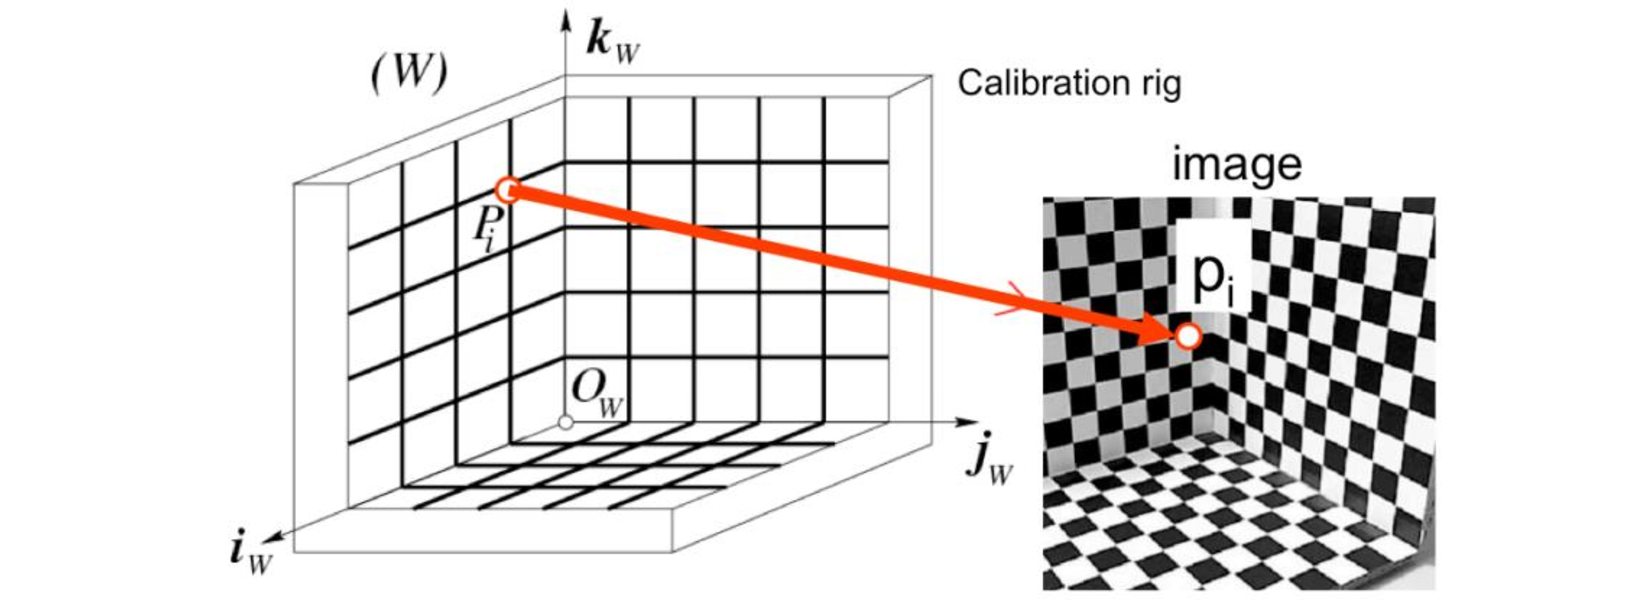
\includegraphics[width=0.8\textwidth]{figures/1-7.pdf}
\caption{The setup of an example calibration rig.}
\label{fig:calibration}
\end{figure}

Specifically, we do this by solving for the intrinsic camera matrix $K$ and the extrinsic parameters $R,T$ from Equation~\ref{eq:cameramatrix}. We can describe this problem in the context of a calibration rig, such as the one show in Figure~\ref{fig:calibration}. The rig usually consists of a simple pattern (i.e. checkerboard) with known dimensions. Furthermore, the rig defines our world reference frame with origin $O_w$ and axes $i_w, j_w, k_w$. From the rig's known pattern, we have known points in the world reference frame $P_1,...,P_n$. Finding these points in the image we take from the camera gives corresponding points in the image $p_1,...,p_n$. 

We set up a linear system of equations from $n$ correspondences such that for each correspondence $P_i, p_i$ and camera matrix $M$ whose rows are $m_1, m_2, m_3$:
\begin{equation}
p_i = \begin{bmatrix}u_i\\v_i\end{bmatrix} = MP_i = \begin{bmatrix}\frac{m_1 P_i}{m_3P_i}\\\frac{m_2 P_i}{m_3P_i}\end{bmatrix}
\end{equation}

As we see from the above equation, each correspondence gives us two equations and, consequently, two constraints for solving the unknown parameters contained in $m$. From before, we know that the camera matrix has $11$ unknown parameters. This means that we need at least $6$ correspondences to solve this. However, in the real world, we often use more, as our measurements are often noisy. To explicitly see this, we can derive a pair of equations that relate $u_i$ and $v_i$ with $P_i$. 
\begin{align*}
u_i(m_3P_i) - m_1P_i = 0\\
v_i(m_3P_i) - m_2P_i = 0
\end{align*}

Given $n$ of these corresponding points, the entire linear system of equations becomes
\begin{align*}
u_1(m_3P_1) -& m_1P_1 = 0\\
v_1(m_3P_1) -& m_2P_1 = 0\\
&\vdots\\
u_n(m_3P_n) -& m_1P_n = 0\\
v_n(m_3P_n) -& m_2P_n = 0\\
\end{align*}

This can be formatted as a matrix-vector product shown below:
\begin{equation}
\begin{bmatrix} 
P_1^T & 0^T & -u_1P_1^T \\
0^T & P_1^T & -v_1P_1^T \\
& \vdots &\\
P_1^T & 0^T & -u_1P_1^T \\
0^T & P_1^T & -v_1P_1^T 
\end{bmatrix}
\begin{bmatrix}
m_1^T \\ m_2^T \\m_3^T
\end{bmatrix} = \mathbf{P}m = 0
\label{eq:linearsystem}
\end{equation}

When $2n > 11$, our homogenous linear system is overdetermined. For such a system $m=0$ is always a trivial solution. Furthemore, even if there were some other $m$ that were a nonzero solution, then $\forall k\in \mathbb{R},km$ is also a solution. Therefore, to constrain our solution, we complete the following minimization:
\begin{equation}
\begin{aligned}
    & \underset{m}{\text{minimize}}
    & & \|\mathbf{P}m\|^2 \\
    & \text{subject to}
    & & \|m\|^2 = 1
\end{aligned}
\end{equation}
To solve this minimization problem, we simply use singular value decomposition. If we let $P = UDV^T$, then the solution to the above minimization is to set $m$ equal to the last column of $V$. The derivation for this solution is outside the scope of this class and you may refer to Section 5.3 of Hartley \& Zisserman on pages 592-593 for more details.

After reformatting the vector $m$ into the matrix $M$, we now want to explicitly solve for the extrinisic and intrisnsic parameters. We know our SVD-solved $M$ is known up to scale, which means that the true values of the camera matrix are some scalar multiple of $M$:
\begin{equation}
M = \rho\begin{bmatrix}
\alpha r_1^T - \alpha\cot \theta r_2^T + u_0r_3^T & \alpha t_x - \alpha \cot \theta t_y + u_0 t_z \\
\frac{\beta}{\sin\theta}r_2^T + v_0r_3^T & \frac{\beta}{\sin\theta}t_y + v_0t_z \\ r_3^T & t_z
\end{bmatrix}
\end{equation}

Dividing by the scaling parameter gives
\[\frac{M}{\rho} = \begin{bmatrix}
\alpha r_1^T - \alpha\cot \theta r_2^T + u_0r_3^T & \alpha t_x - \alpha \cot \theta t_y + u_0 t_z \\
\frac{\beta}{\sin\theta}r_2^T + v_0r_3^T & \frac{\beta}{\sin\theta}t_y + v_0t_z \\ r_3^T & t_z
\end{bmatrix} = \begin{bmatrix}A & b\end{bmatrix} =\begin{bmatrix}
a_1^T \\ a_2^T \\ a_3^T
\end{bmatrix} \begin{bmatrix}
b_1\\b_2\\b_3
\end{bmatrix}
\]

Solving for the intrinsics gives 
\begin{equation}\begin{aligned}
    \rho &= \pm \frac{1}{\|a_3\|}\\
    u_o &= \rho^2(a_1\cdot a_3)\\
    v_o &=\rho^2(a_2\cdot a_3)\\
    \theta &= \cos ^{-1} \frac{(a_1 \times a_3)\cdot(a_2\times a_3)}{\|a_1\times a_3\|\cdot\|a_2\times a_3\|}\\
    \alpha &= \rho^2 \|a_1 \times a_3\| \sin \theta\\
    \beta &= \rho^2 \|a_2 \times a_3\| \sin \theta
\end{aligned}\end{equation}

The extrinsics are 
\begin{equation}\begin{aligned}
    r_1 &= \frac{a_2\times a_3}{\|a_2\times a_3\|}\\
    r_2 &= r_3\times r_1\\
    r_3 &= \pm \frac{ a_3}{\| a_3\|}\\
    T &= \rho K^-1 b
\end{aligned}\end{equation}
We leave the derivations as a class exercise or you can refer to Section 1.3.1 of the Forsyth \& Ponce textbook.

With the calibration procedure complete, we warn against degenerate cases. Not all sets of $n$ correspondences will work. For example, if the points $P_i$ lie on the same plane, then the system will not be able to be solved. These unsolvable configurations of points are known as \emph{degenerate configurations}. More generally, degenerate configurations have points that lie on the intersection curve of two quadric surfaces. Although this outside the scope of the class, you can find more information in Section 1.3 of the Forsyth \& Ponce textbook. 

\section{Handling Distortion in Camera Calibration}
So far, we have been working with ideal lenses which are free from any distortion. However, as seen before, real lenses can deviate from rectilinear projection, which require more advanced methods. This section provides just a brief introduction to handling distortions. 

Often, distortions are radially symmetric because of the physical symmetry of the lens. We model the radial distortion with an isotropic transformation:
\begin{equation}
    QP_i = \begin{bmatrix}
    \frac{1}{\lambda}&0&0\\0 &    \frac{1}{\lambda} & 0 \\ 0 & 0 &1\end{bmatrix} M P_i = \begin{bmatrix}
    u_i\\v_i\end{bmatrix}
    = p_i
\end{equation}
If we try to rewrite this into a system of equations as before, we get 

\begin{align*}
    u_iq_3P_i  = q_1P_i\\
    v_iq_3P_i  = q_2P_i
\end{align*}

This system, however, is no longer linear, and we require the use nonlinear optimization techniques, which are covered in Section 22.2 of Forsyth \& Ponce. We can simplify the nonlinear optimization of the calibration problem if we make certain assumptions. In radial distortion, we note that the ratio between two coordinates $u_i$ and $v_i$ is not affected. We can compute this ratio as
\begin{equation}
    \frac{u_i}{v_i} = \frac{\frac{m_1P_i}{m_3P_i}}{\frac{m_2P_i}{m_3P_i}} = \frac{m_1P_i}{m_2P_i}
\end{equation}

Assuming that $n$ correspondences are available, we can set up the system of linear equations:
\begin{align*}
    v_1(m_1P_1)-&u_1(m_2P_1) = 0\\
    &\vdots\\
    v_n(m_1P_n)-&u_n(m_2P_n) = 0
\end{align*}
Similar to before, this gives a matrix-vector product that we can solve via SVD:
\begin{equation}
    Ln = \begin{bmatrix}
    v_1P_1^T & -u_1P_1^T\\
    \vdots & \vdots\\
    v_nP_n^T & -u_nP_n^T\\ 
    \end{bmatrix}
    \begin{bmatrix}
    m_1^T\\m_2^T
    \end{bmatrix}
\end{equation}

Once $m_1$ and $m_2$ are estimated, $m_3$ can be expressed as a nonlinear function of $m_1,m_2,$ and $\lambda$. This requires to solve a nonlinear optimization problem whose complexity is much simpler than the original one.

\section{Appendix A: Rigid Transformations}
The basic rigid transformations are rotation, translation, and scaling. This appendix will cover them for the 3D case, as they are common type in this class. 

Rotating a point in 3D space can be represented by rotating around each of the three coordinate axes respectively. When rotating around the coordinate axes, common convention is to rotate in a counter-clockwise direction. One intuitive way to think of rotations is how much we rotate around each degree of freedom, which is often referred to as \emph{Euler angles}. However, this methodology can result in what is known as \emph{singularities}, or \emph{gimbal lock}, in which certain configurations result in a loss of a degree of freedom for the rotation. 

One way to prevent this is to use rotation matrices, which are a more general form of representing rotations. Rotation matrices are square, orthogonal matrices with determinant one. Given a rotation matrix $R$ and a vector $v$, we can compute the resulting vector $v'$ as
\[v' = Rv\]

Since rotation matrices are a very general representation of matrices, we can represent a rotation $\alpha, \beta, \gamma$ around each of the respective axes as follows:
\[R_x(\alpha) = \begin{bmatrix}1 & 0 & 0\\ 0 &\cos\alpha &-\sin\alpha \\ 0 &\sin\alpha &\cos\alpha \end{bmatrix}\]
\[R_y(\beta) = \begin{bmatrix}\cos\beta & 0 & \sin\beta \\ 0 & 1 & 0 \\ -\sin\beta & 0 &\cos\beta \end{bmatrix}\]
\[R_z(\gamma) = \begin{bmatrix}\cos \gamma & -\sin\gamma &0 \\ \sin\gamma &\cos\gamma & 0 \\ 0 & 0 & 1 \end{bmatrix}\]

Due to the convention of matrix multiplication, the rotation achieved by first rotating around the z-axis, then y-axis, then x-axis is given by the matrix product $R_xR_yR_z$.

Translations, or displacements, are used to describe the movement in a certain direction. In 3D space, we define a translation vector $t$ with 3 values: the displacements in each of the 3 axes, often denoted as $t_x, t_y, t_z$. Thus, given some point $P$ which is translated to some other point $P'$ by $t$, we can write it as:
\[ P' = P + t = \begin{bmatrix}P_x\\P_y\\P_z\end{bmatrix} + \begin{bmatrix}t_x\\t_y\\t_z\end{bmatrix}\]

In matrix form, translations can be written using homogeneous coordinates. If we construct a translation matrix as
\[ T = \begin{bmatrix}
1 & 0 & 0 & t_x \\0 & 1 & 0 & t_y \\0 & 0 & 1 & t_z \\ 0 & 0 & 0 & 1
\end{bmatrix}\]
then we see that $P'=TP$ is equivalent to $P' = P+t$.


If we want to combine translation with our rotation matrix multiplication, we can again use homogeneous coordinates to our advantage. If we want to rotate a vector $v$ by $R$ and then translate it by $t$, we can write the resulting vector $v'$ as:
\[ \begin{bmatrix}v'\\1\end{bmatrix} = \begin{bmatrix}
R & t \\ 0 & 1
\end{bmatrix}\begin{bmatrix}
v \\ 1
\end{bmatrix}\]

Finally, if we want to scale the vector in certain directions by some amount $S_x, S_y, S_z$, we can construct a scaling matrix 
\[S = \begin{bmatrix}
S_x & 0 & 0 \\ 0 & S_y & 0 \\ 0 & 0 & S_z
\end{bmatrix}\]

Therefore, if we want to scale a vector, then rotate, then translate, our final transformation matrix would be:
\[T = \begin{bmatrix}
RS & t \\ 0 & 1
\end{bmatrix}\]

Note that all of these types of transformations would be examples of affine transformations. Recall that projective transformations occur when the final row of $T$ is not $\begin{bmatrix}
0 & 0 &0 &1
\end{bmatrix}$.

\section{Appendix B: Different Camera Models}
We will now describe a simple model known as the \emph{weak perspective model}. In the weak perspective model, points are first projected to the reference plane using orthogonal projection and then projected to the image plane using a projective transformation.
\begin{figure}[h!]
\centering
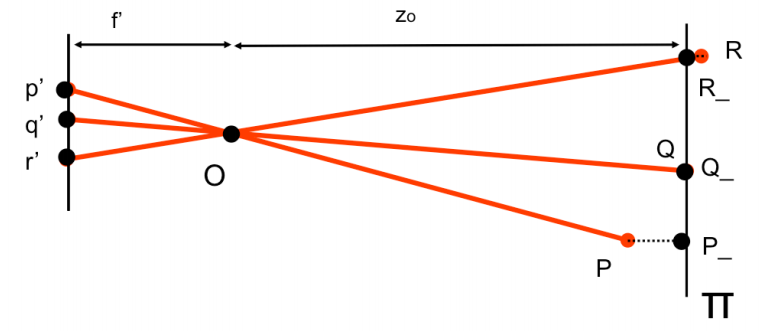
\includegraphics[width=0.8\textwidth]{figures/weak_perspective.png}
\caption{The weak perspective model: orthogonal projection onto reference plane}
\label{fig:weak_perspective}
\end{figure}

As Figure~\ref{fig:weak_perspective} shows, given a reference plane $\Pi$ at a distance $z_o$ from the center of the camera, the points $P,Q,R$ are first projected to the plane $\Pi$ using an orthogonal projection, generating points $P\_, Q\_, R\_$.  This is a reasonable approximation when deviations in depth from the plane are small compared to the distance of the camera. 

\begin{figure}[h!]
\centering
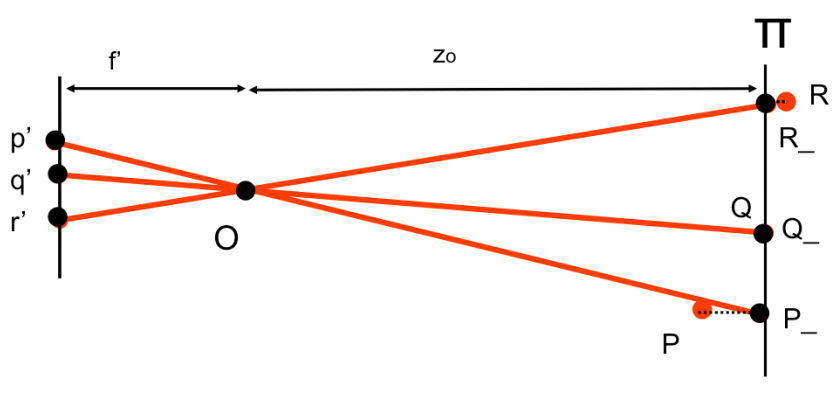
\includegraphics[width=0.8\textwidth]{figures/weak_perspective2.png}
\caption{The weak perspective model: projection onto the image plane}
\label{fig:weak_perspective2}
\end{figure}

Figure~\ref{fig:weak_perspective2} illustrates how points $P\_, Q\_, R\_$ are then projected to the image plane using a regular projective transformation to produce the points $p', q', r'$. Notice, however, that because we have approximated the depth of each point to $z_o$ the projection has been reduced to a simple, constant magnification. The magnification is equal to the focal length $f'$ divided by $z_o$, leading to
\begin{align*}
x'=\frac{f'}{z_0}x\ \ \ \ \ 
y'=\frac{f'}{z_0}y
\end{align*}
This model also simplifies the projection matrix
\[M = \begin{bmatrix}
A & b \\ 0 & 1
\end{bmatrix}\]
As we see, the last row of $M$ is $\begin{bmatrix}
0 & 0& 0 &1
\end{bmatrix}$ in the weak perspective model, compared to $\begin{bmatrix}
v&1
\end{bmatrix}$ in the normal camera model. We do not prove this result and leave it to you as an exercise. The simplification is clearly demonstrated when mapping the 3D points to the image plane. 
\begin{equation}
    P' = MP = \begin{bmatrix}
    m_1 \\ m_2 \\ m_3
    \end{bmatrix}P = \begin{bmatrix}
    m_1P \\ m_2P \\ 1
    \end{bmatrix}
\end{equation}
Thus, we see that the image plane point ultimately becomes a magnification of the original 3D point, irrespective of depth. The nonlinearity of the projective transformation disappears, making the weak perspective transformation a mere magnifier.

\begin{figure}[h!]
\centering
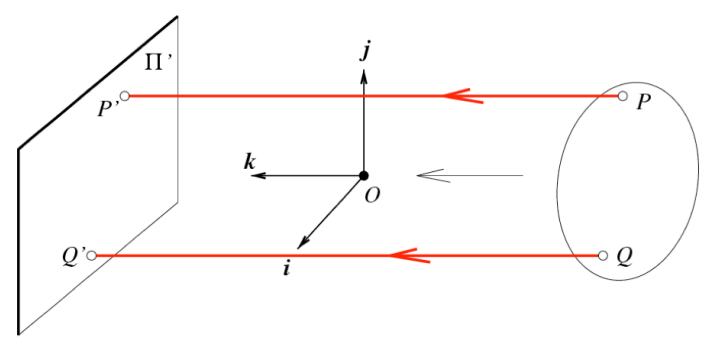
\includegraphics[width=0.8\textwidth]{figures/orthographic.png}
\caption{The orthographic projection model}
\label{fig:orthographic}
\end{figure}


Further simplification leads to the \emph{orthographic (or affine) projection model}. In this case, the optical center is located at infinity. The projection rays are now perpendicular to the retinal plane. As a result, this model ignores depth altogether.  Therefore,
\begin{align*}
    x' = x\\
    y' = y
\end{align*}
Orthographic projection models are often used for architecture and industrial design.

Overall, weak perspective models result in much simpler math, at the cost of being somewhat imprecise. However, it often yields results that are very accurate when the object is small and distant from the camera. 
\end{document}
